% ----------------------------------------------------------------------

\newpage

\subsection{\scurves Test}
\label{ss:scurves}

\subsubsection{Purpose}

The \scurves test has two primary purposes.
First, it evaluates the efficacy of the \trimming test.
Secondly, it measures the noise present in each pixel and can potentially flag abnormally noisy pixels.
Both of these goals are achieved by fitting the curve of efficiency vs. \vcal for each pixel.
The test gets its name from the shape of the error function used to fit the measured curve.

\subsubsection{\textcolor{red}{Methodology}}

\subsubsection{Output}

\begin{figure}[!Hp]
\centering
\begin{minipage}{0.45\textwidth}
  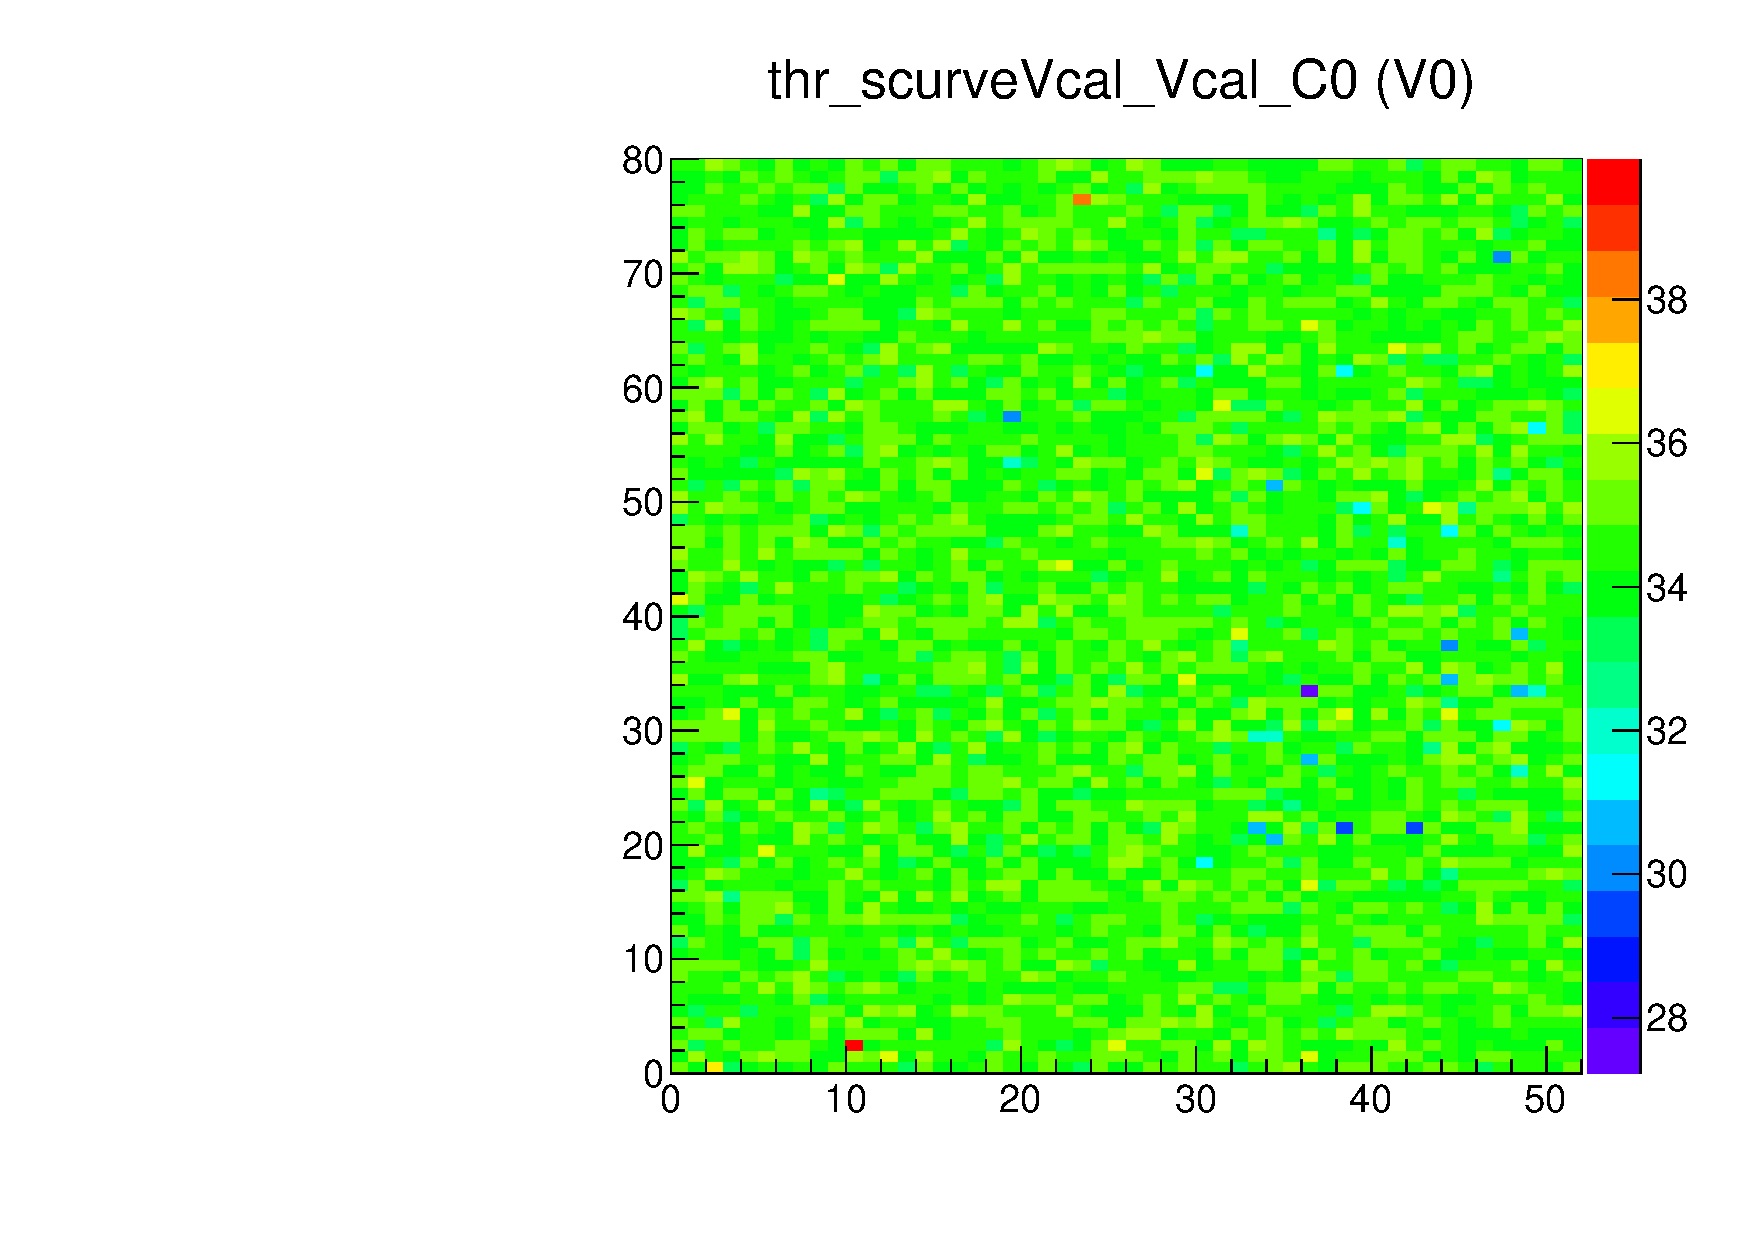
\includegraphics[width=1.0\textwidth]{figures/scurves_thr_scurveVcal_Vcal.pdf}
  \caption{\roc map of the \vcal s-curve turn-on thresholds.
  Values should be near the trim target (default 35).}
  \label{fig:scurves_thr_scurveVcal_Vcal}
\end{minipage}
\hspace{0.3cm}
\begin{minipage}{0.45\textwidth}
  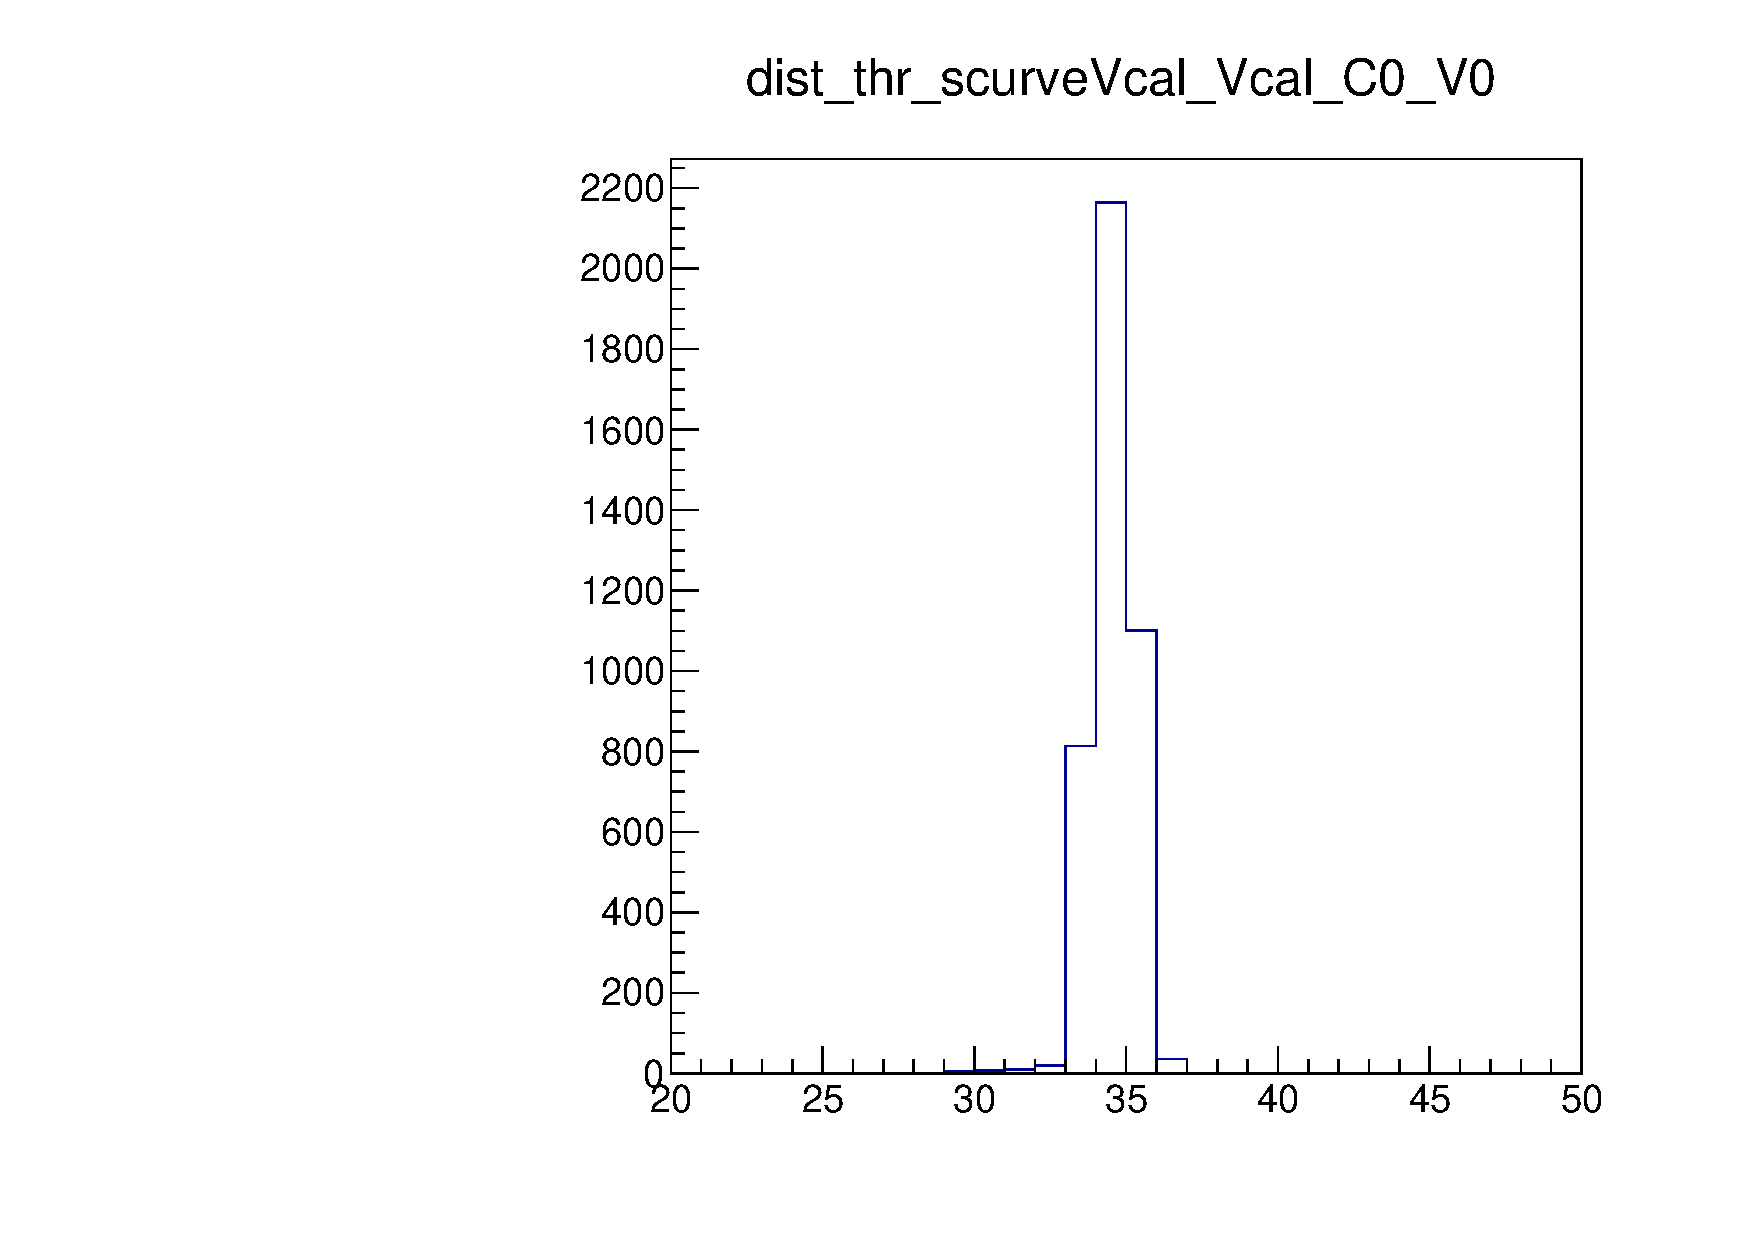
\includegraphics[width=1.0\textwidth]{figures/scurves_dist_thr_scurveVcal_Vcal.pdf}
  \caption{1D distribution of Figure~\ref{fig:scurves_thr_scurveVcal_Vcal}.
  [original range 0-255]}
  \label{fig:scurves_dist_thr_scurveVcal_Vcal}
\end{minipage}
\end{figure}

\begin{figure}[!Hp]
\centering
\begin{minipage}{0.45\textwidth}
  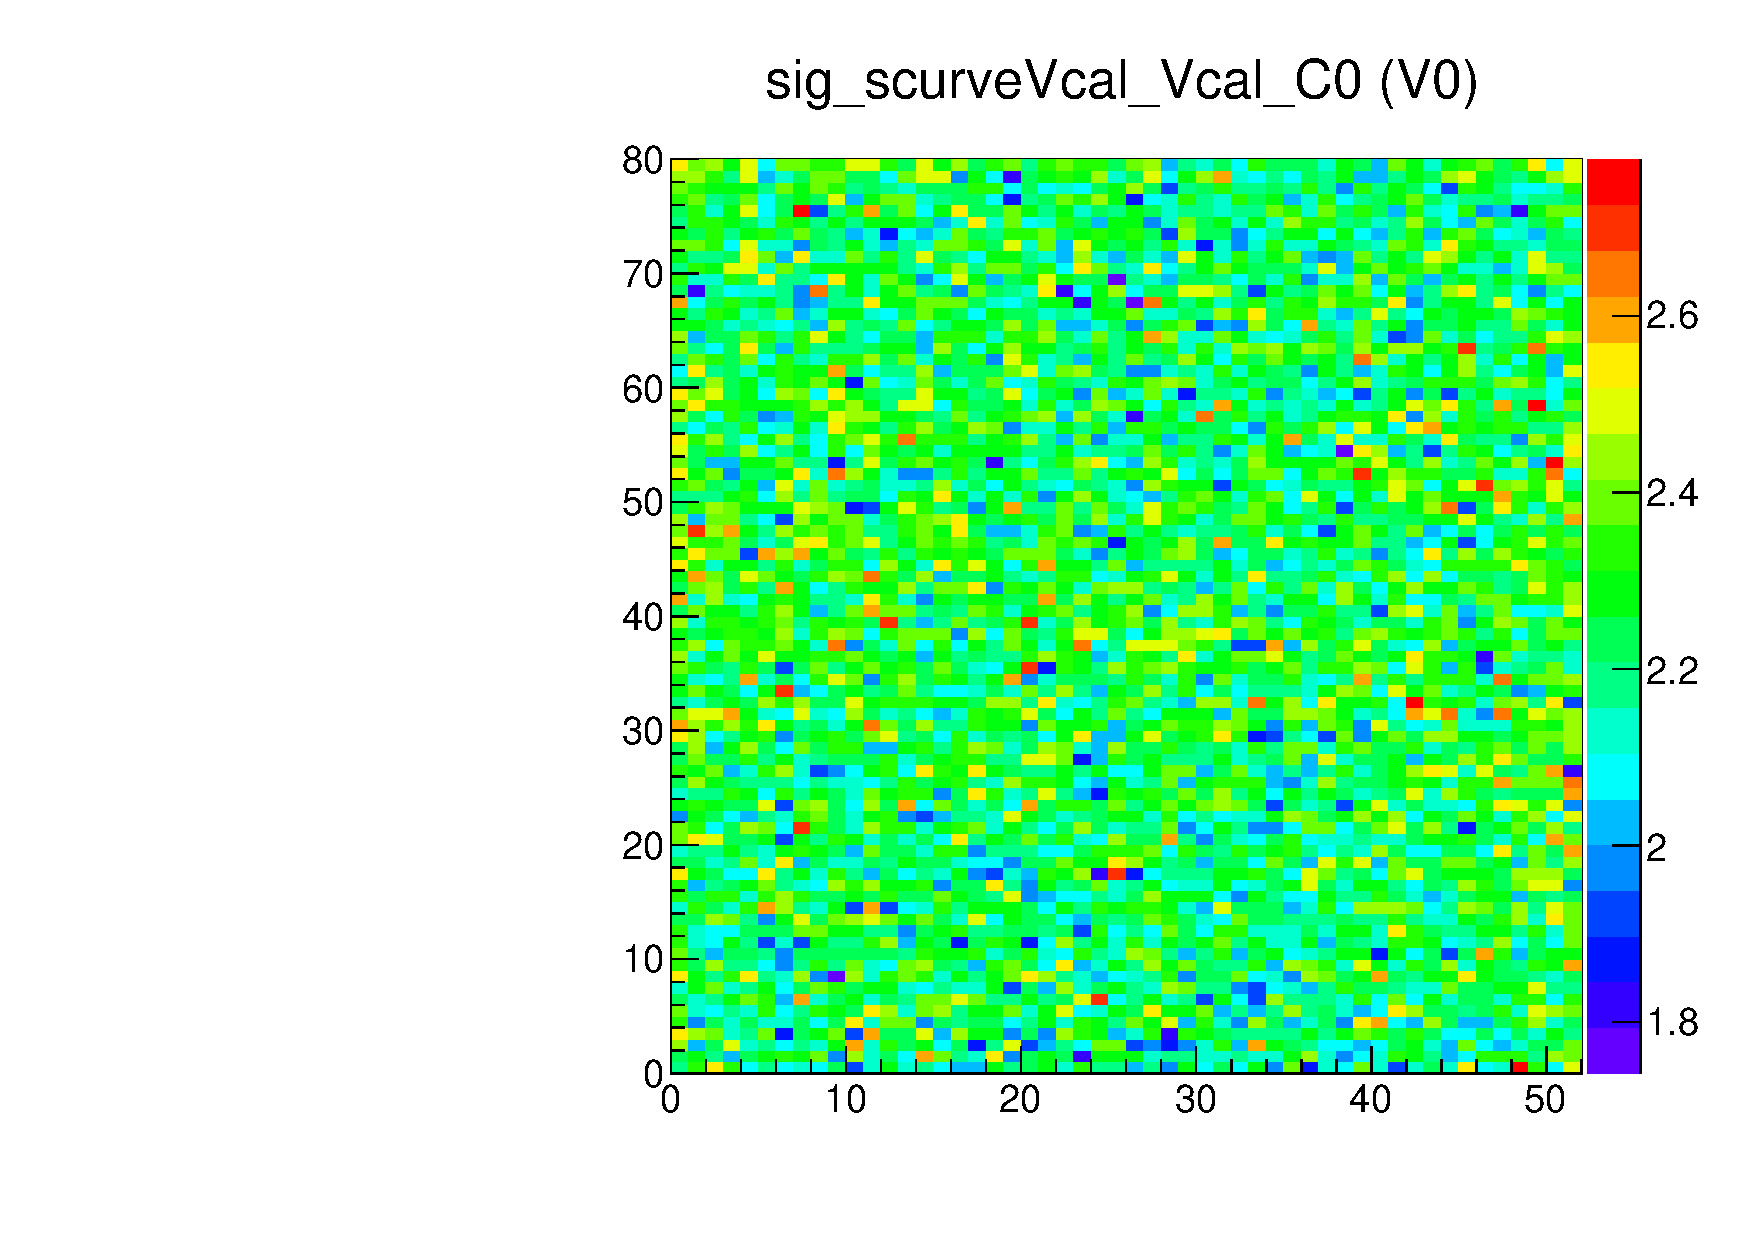
\includegraphics[width=1.0\textwidth]{figures/scurves_sig_scurveVcal_Vcal.pdf}
  \caption{\roc map of the \vcal s-curve turn-on widths.  
  This width is proportional to the noise in the system.}
  \label{fig:scurves_sig_scurveVcal_Vcal}
\end{minipage}
\hspace{0.3cm}
\begin{minipage}{0.45\textwidth}
  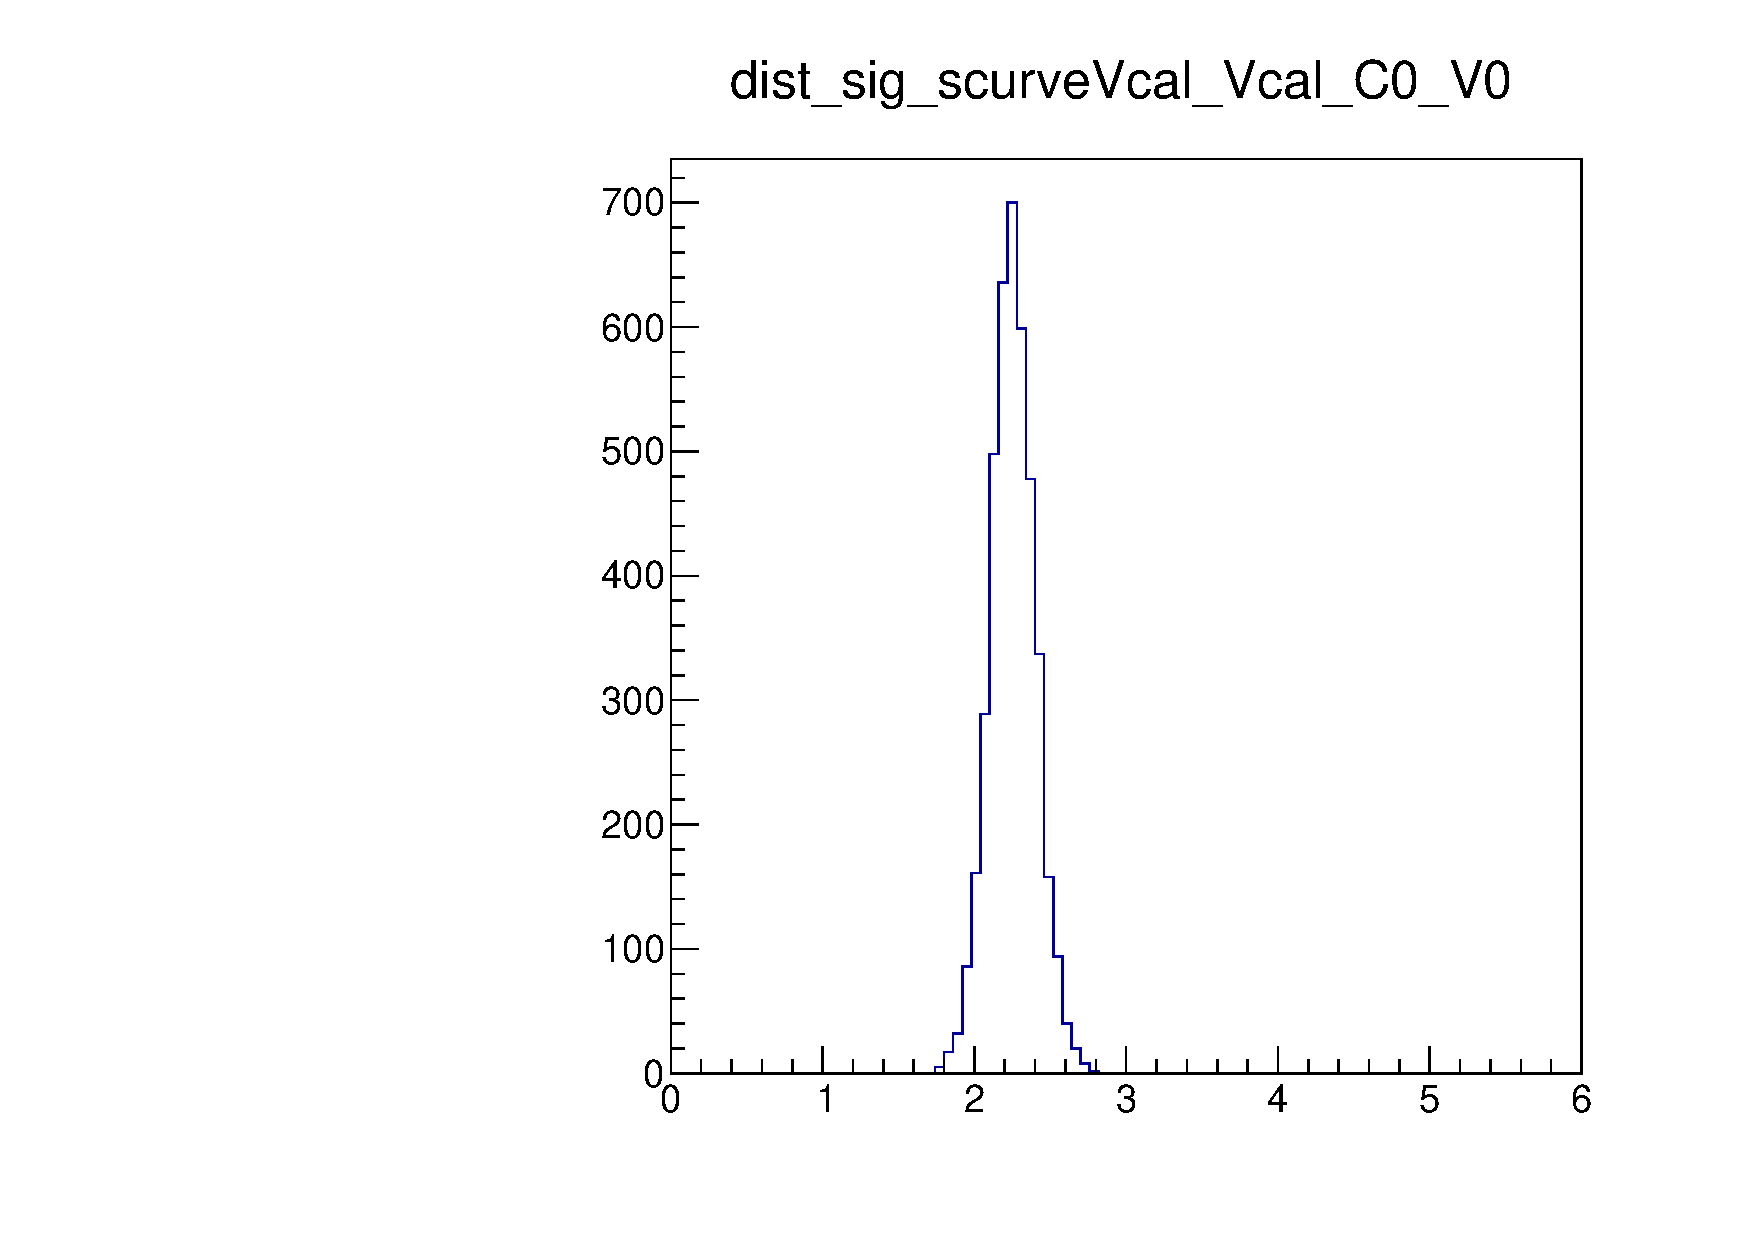
\includegraphics[width=1.0\textwidth]{figures/scurves_dist_sig_scurveVcal_Vcal.pdf}
  \caption{1D distribution of Figure~\ref{fig:scurves_sig_scurveVcal_Vcal}.}
  \label{fig:scurves_dist_sig_scurveVcal_Vcal}
\end{minipage}
\end{figure}

\begin{figure}[!Hp]
\centering
\begin{minipage}{0.45\textwidth}
  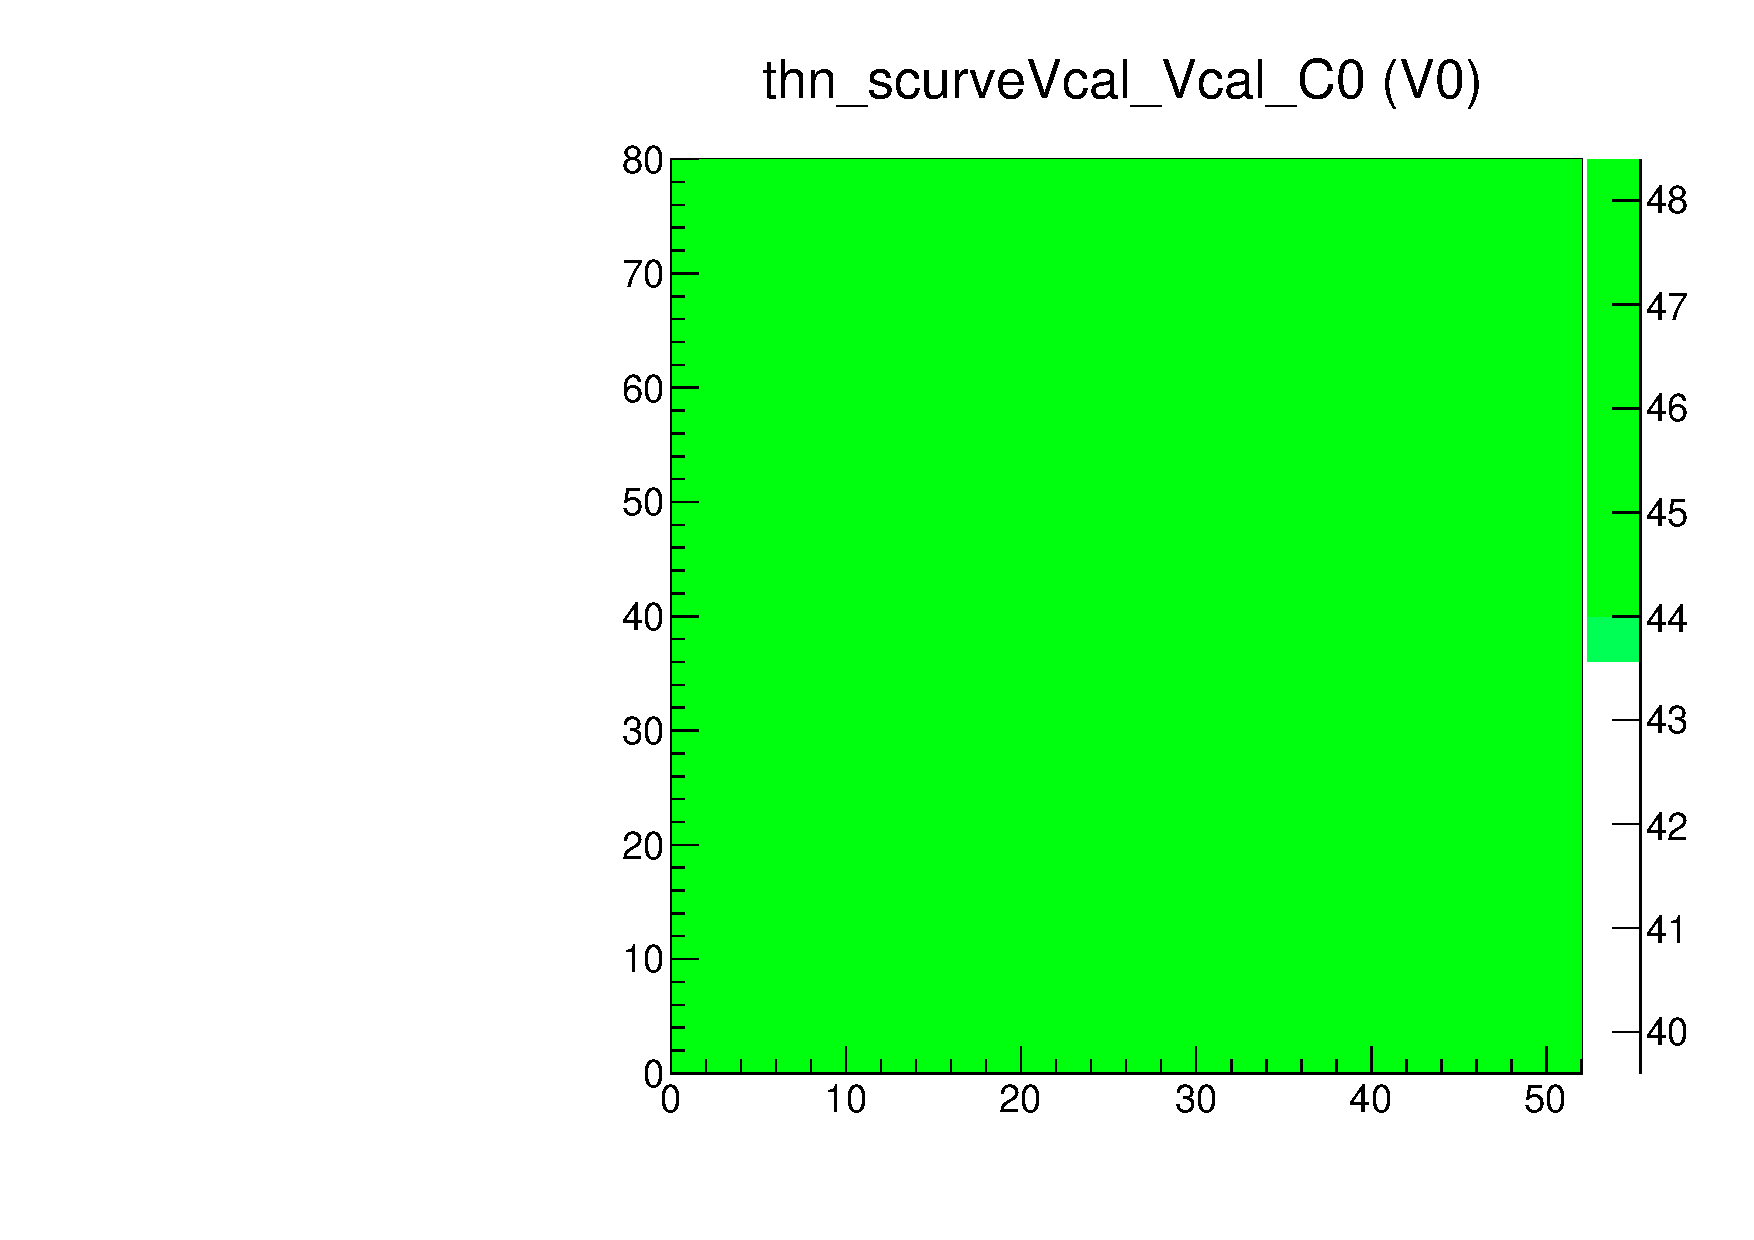
\includegraphics[width=1.0\textwidth]{figures/scurves_thn_scurveVcal_Vcal.pdf}
  \caption{\roc map of the \vcal s-curve turn-off thresholds.  
  For s-curves with respect to \vcal, no turn off is expected.
  Therefore this plot should be uniformly distributed at the maximum value of \vcal considered by the test.}
  \label{fig:scurves_thn_scurveVcal_Vcal}
\end{minipage}
\hspace{0.3cm}
\begin{minipage}{0.45\textwidth}
  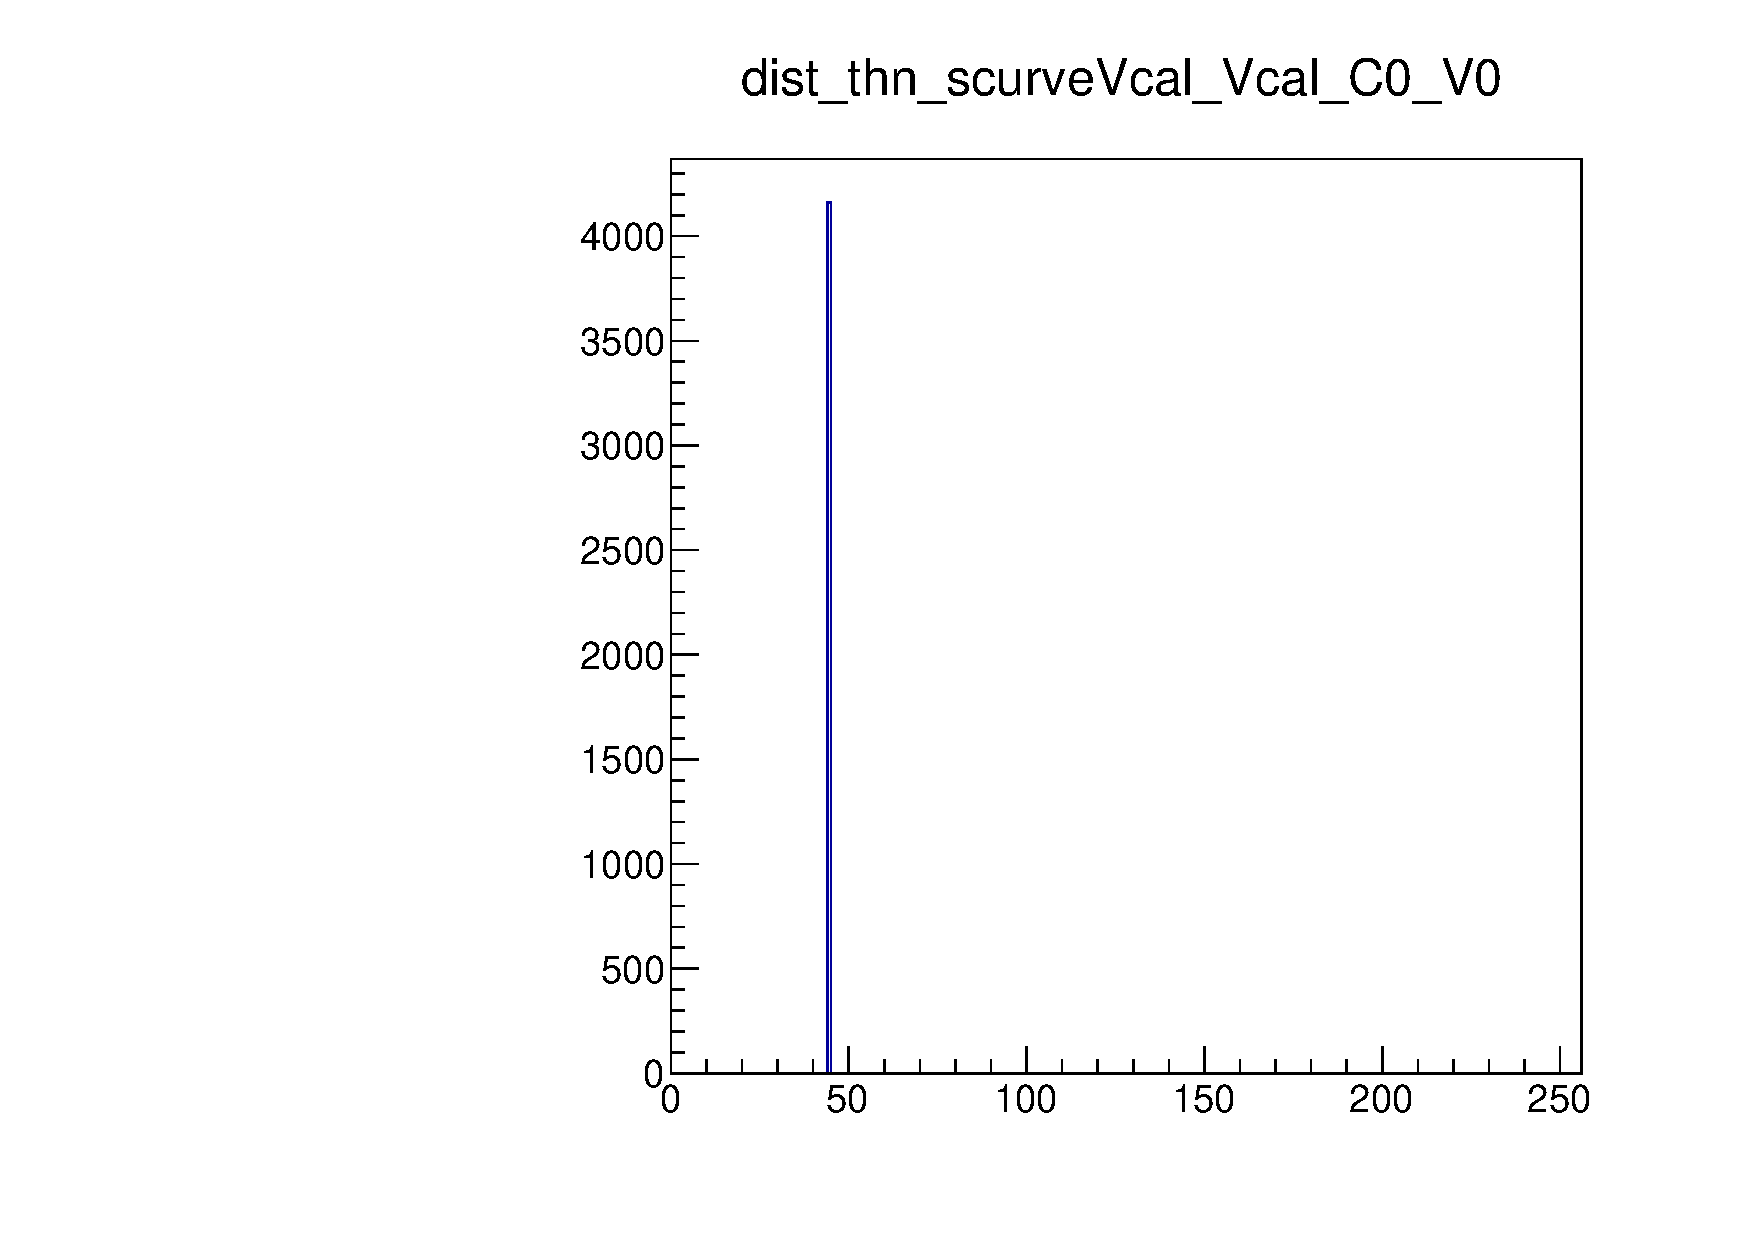
\includegraphics[width=1.0\textwidth]{figures/scurves_dist_thn_scurveVcal_Vcal.pdf}
  \caption{1D distribution of Figure~\ref{fig:scurves_thn_scurveVcal_Vcal}.}
  \label{fig:scurves_dist_thn_scurveVcal_Vcal}
\end{minipage}
\end{figure}


